\section{Bins size}
\label{sec:binning}
The choice of bins size in the variables $W$, $Q^2$, $\cos\theta^*$, $\phi^*$
is illustrated in Fig. \ref{fig:binning1} and Fig. \ref{fig:binning2}.
The bin sizes were chosen to agree with previous and ongoing analyses.


$W$ was divided in $15$ bins from $1.1$ GeV to $1.4$ GeV in step of
$\Delta W = 0.02$ $GeV$. $\Delta Q^2$ is variable and such that $\Delta Q^2/Q^2\simeq 0.18$. 
The values are in table \ref{tab:binning}.

\begin{figure}[h]
 \begin{center}
  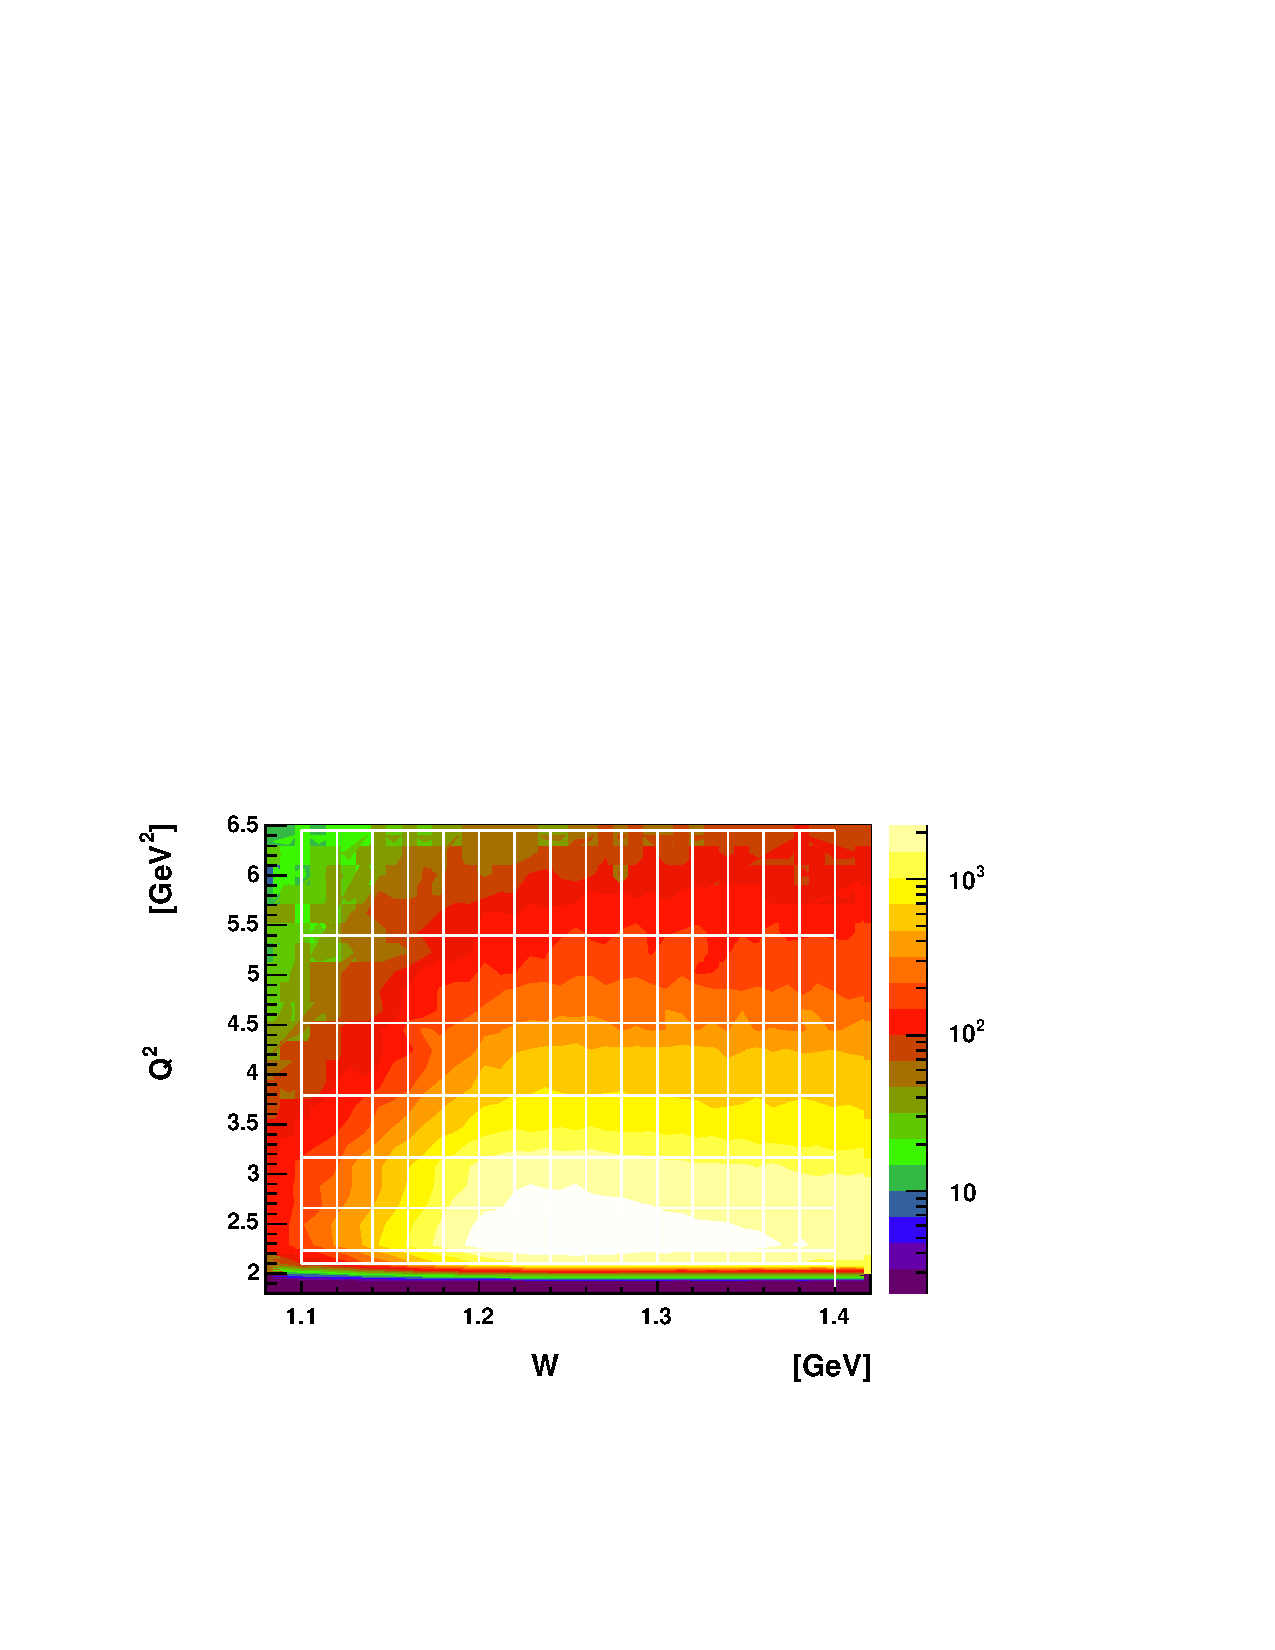
\includegraphics[width=12cm, bb=40 140 520 460]{analysis/img/binning1}
  \caption[$W$ and $Q^2$ binning for $\pi^0$ events]
          { $W$ and $Q^2$ binning for $\pi^0$ events (all angles). Notice the increasing $\Delta Q^2$ size with $Q^2$.}
 \label{fig:binning1}
  \end{center} 
\end{figure} 


\begin{table}[h]
 \begin{center}
  \begin{tabular}{|l|c|c|c|c|c|c|c|}
    \hline 
   $Q^2$        & 2.15  & 2.4  & 3.0  & 3.5  & 4.2  & 5.0  & 6.0 \\ 
    \hline  
   $Q^2_{min}$  & 2.10 & 2.23 & 2.66 & 3.17 & 3.79 & 4.52 & 5.40 \\
   \hline
   $Q^2_{max}$  & 2.23 & 2.66 & 3.17 & 3.79 & 4.52 & 5.40 & 6.45\\       
 \hline
  \end{tabular}
 \end{center} 
 \caption[The binning in $Q^2$]
         { The binning in $Q^2$.}
 \label{tab:binning}
\end{table}

The angular bins are taken as follows:
$\Delta \cos\theta^* = 0.2$ and $\Delta\phi^* = 30^0$ so that there are $10$ bins in  $\cos\theta^*$ and $12$ in $\phi^*$
as shown in  Fig. \ref{fig:binning2}.
\begin{figure}[h]
 \begin{center}
  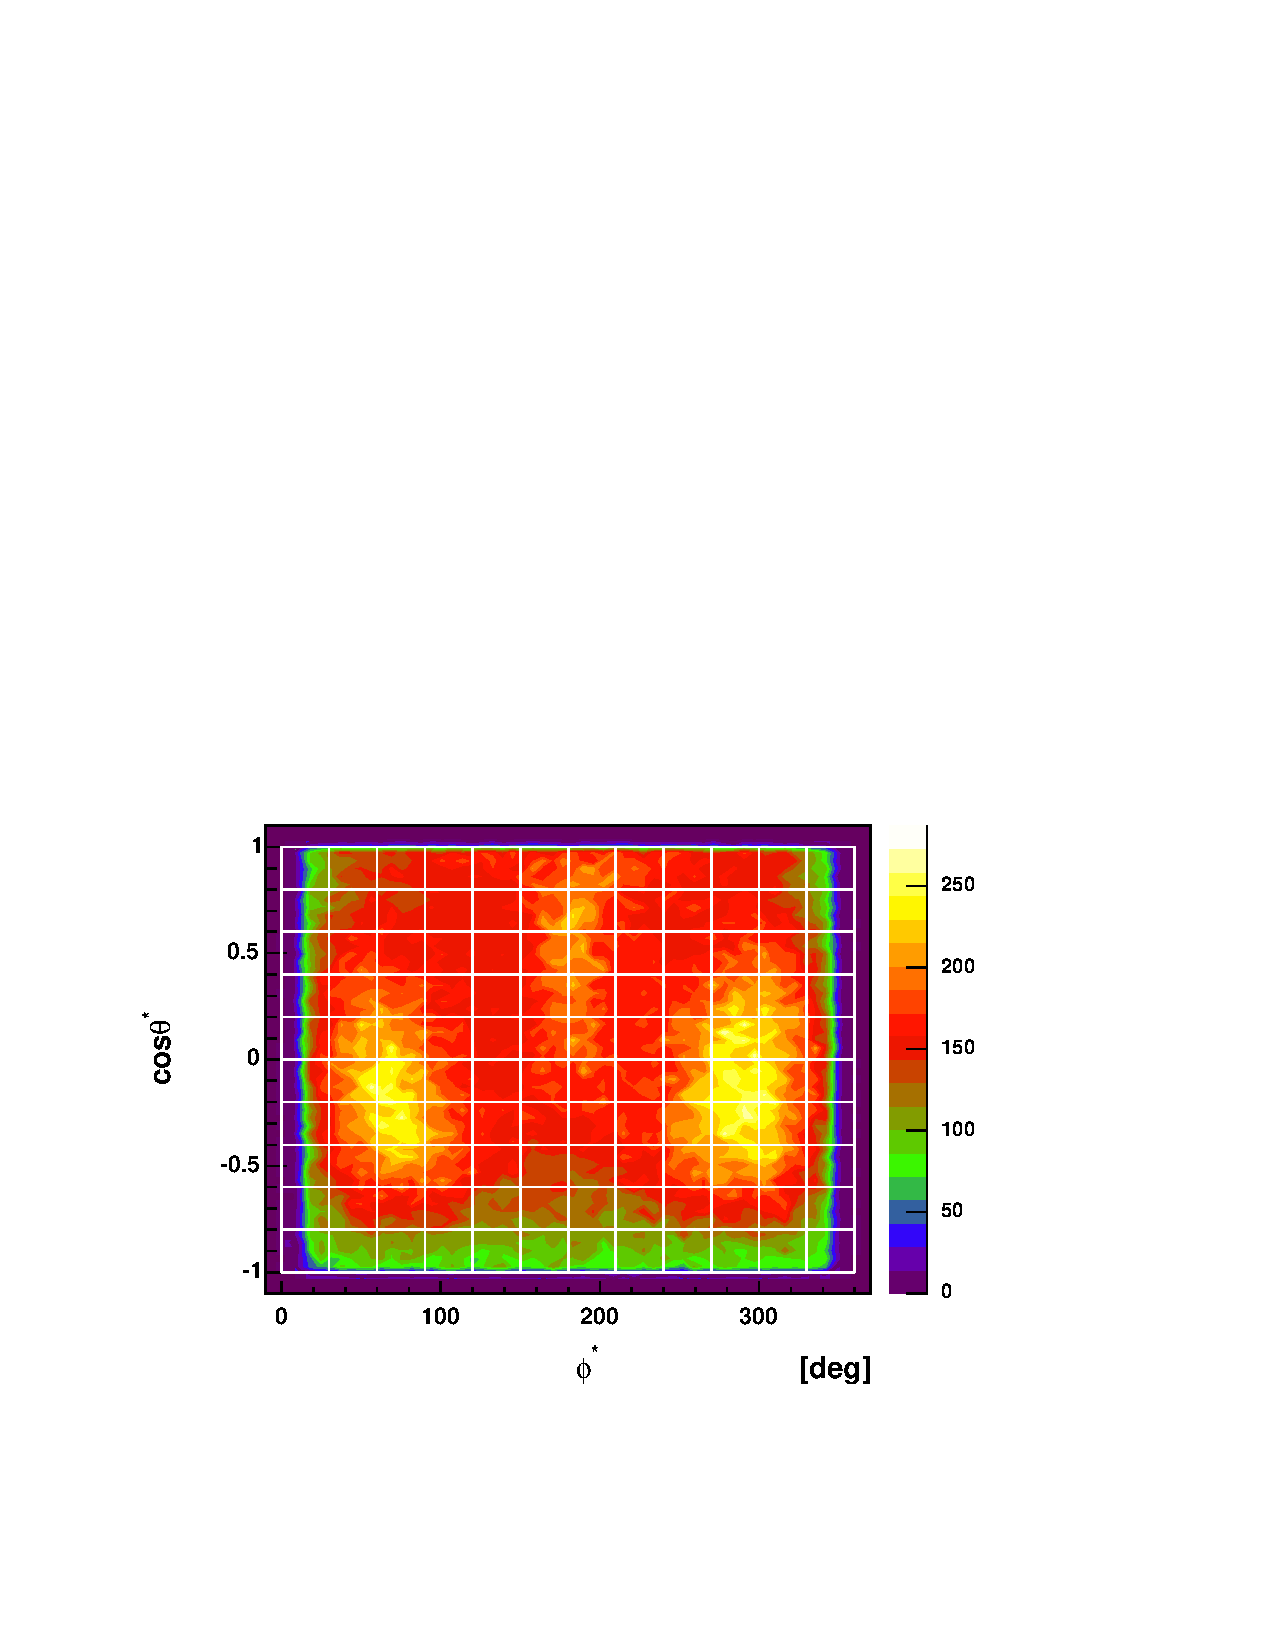
\includegraphics[width=12cm, bb=60 120 480 460]{analysis/img/binning2}
  \caption[$\cos\theta^*$ and $\phi^*$ binning for $\pi^0$ events]
          { $\cos\theta^*$ and $\phi^*$ binning for $\pi^0$ events (all $W$ and $Q^2$).}
 \label{fig:binning2}
\end{center} 
\end{figure}









